\documentclass[12pt,a4paper]{article}

% ─── Page Layout ───────────────────────────────────────────────────────────────
\usepackage[a4paper, margin=0.8in, headheight=14pt]{geometry}

% ─── Fonts (XeLaTeX) ───────────────────────────────────────────────────────────
\usepackage{fontspec}
\usepackage{unicode-math}
\setmainfont{TeX Gyre Pagella}
\setmonofont[Scale=0.88]{TeX Gyre Cursor}
\setmathfont{Latin Modern Math}

% ─── Packages ──────────────────────────────────────────────────────────────────
\usepackage{xcolor}
\usepackage{colortbl}
\usepackage{titlesec}
\usepackage{enumitem}
\usepackage{tabularx}
\usepackage{booktabs}
\usepackage{array}
\usepackage{amsmath}
\usepackage{tikz}
\usetikzlibrary{shapes.geometric, arrows.meta, positioning, calc, fit, decorations.pathreplacing}
\usepackage{tcolorbox}
\tcbuselibrary{skins, breakable}
\usepackage{hyperref}
\usepackage{fancyhdr}
\usepackage{graphicx}
\usepackage{microtype}
\hyphenpenalty=10000
\exhyphenpenalty=10000
\sloppy
\usepackage{caption}
\usepackage{setspace}
\usepackage{multirow}
\usepackage{tocloft}

% ─── Q&A helper ────────────────────────────────────────────────────────────────
\newcommand{\Q}[1]{\textbf{#1}\par\noindent\ignorespaces}

% ─── Colour Palette ────────────────────────────────────────────────────────────
\definecolor{myred}{RGB}{196,30,58}
\definecolor{mydark}{RGB}{30,30,50}
\definecolor{mygreen}{RGB}{14,120,80}
\definecolor{myteal}{RGB}{0,130,140}
\definecolor{myamber}{RGB}{180,100,0}
\definecolor{mypurple}{RGB}{100,30,160}
\definecolor{mygray}{RGB}{246,247,249}
\definecolor{mgframe}{RGB}{180,185,200}
\definecolor{watermark}{RGB}{145,150,170}
\definecolor{hdrred}{RGB}{250,232,235}
\definecolor{hdrgreen}{RGB}{220,244,233}
\definecolor{hdrteal}{RGB}{220,242,244}
\definecolor{hdramber}{RGB}{253,242,215}
\definecolor{hdrpurple}{RGB}{238,228,255}
\definecolor{hdrgray}{RGB}{238,240,245}
\definecolor{rowalt}{RGB}{250,251,253}

% ─── Section Formatting ────────────────────────────────────────────────────────
\titleformat{\section}
  {\large\bfseries\color{myred}}{\thesection.}{0.5em}{}
  [\vspace{1pt}{\color{myred}\rule{\linewidth}{0.8pt}}]
\titleformat{\subsection}
  {\normalsize\bfseries\color{myteal}}{\thesubsection}{0.5em}{}
\titlespacing*{\section}{0pt}{18pt}{7pt}
\titlespacing*{\subsection}{0pt}{11pt}{4pt}

% ─── Paragraph ─────────────────────────────────────────────────────────────────
\setlength{\parindent}{0pt}
\setlength{\parskip}{4pt}

% ─── TOC Styling ───────────────────────────────────────────────────────────────
\renewcommand{\cfttoctitlefont}{\large\bfseries\color{myred}}
\renewcommand{\cftaftertoctitle}{\par\noindent{\color{myred}\rule{\linewidth}{0.8pt}}}
\setlength{\cftbeforetoctitleskip}{0pt}
\setlength{\cftaftertoctitleskip}{6pt}
\renewcommand{\cftsecfont}{\normalsize\bfseries\color{mydark}}
\renewcommand{\cftsecpagefont}{\normalsize\bfseries\color{mydark}}
\renewcommand{\cftsecleader}{\cftdotfill{\cftdotsep}}
\setlength{\cftbeforesecskip}{7pt}
\renewcommand{\cftsubsecfont}{\small\color{mydark}}
\renewcommand{\cftsubsecpagefont}{\small\color{mydark}}
\setlength{\cftbeforesubsecskip}{3pt}
\setlength{\cftsubsecindent}{1.4em}

% ─── Table helpers ─────────────────────────────────────────────────────────────
\renewcommand{\arraystretch}{1.45}
\setlength{\tabcolsep}{6pt}
\arrayrulecolor{mydark}
\newcolumntype{B}[1]{>{\small\bfseries\raggedright\arraybackslash}m{#1}}
\newcolumntype{Y}{>{\small\raggedright\arraybackslash}X}
\renewcommand{\tabularxcolumn}[1]{m{#1}}

% ─── Header / Footer ───────────────────────────────────────────────────────────
\pagestyle{fancy}
\fancyhf{}
\fancyhead[L]{\small\color{myred}\textbf{PE-EC701B}\;\color{mydark}--- Satellite Communication}
\fancyhead[R]{\small\color{myteal}\textbf{Module 2 Notes}}
\fancyfoot[C]{\small\color{mydark}\thepage}
\fancyfoot[R]{\small\color{watermark}\textit{\copyright\ Biraj}}
\renewcommand{\headrulewidth}{0.5pt}
\renewcommand{\footrulewidth}{0.3pt}

% ─── Hyperref ──────────────────────────────────────────────────────────────────
\hypersetup{
  colorlinks=true, linkcolor=myteal, urlcolor=myteal,
  pdfauthor={Biraj Sarkar},
  pdftitle={PE-EC701B --- Module 2 Notes}
}

% ─── tcolorbox styles ──────────────────────────────────────────────────────────
\tcbset{
  tikzbox/.style={
    colback=mygray, colframe=mgframe, boxrule=0.6pt, arc=4pt,
    left=8pt, right=8pt, top=6pt, bottom=6pt,
    colbacktitle=mgframe, coltitle=mydark,
    fonttitle=\small\bfseries
  },
  defbox/.style={
    colback=hdrgreen, colframe=mygreen, boxrule=0.8pt, arc=4pt,
    left=9pt, right=9pt, top=6pt, bottom=6pt,
    colbacktitle=mygreen, coltitle=white,
    fonttitle=\small\bfseries
  },
  formulabox/.style={
    colback=hdrteal, colframe=myteal, boxrule=0.8pt, arc=4pt,
    left=9pt, right=9pt, top=7pt, bottom=7pt,
    colbacktitle=myteal, coltitle=white,
    fonttitle=\small\bfseries
  },
  examplebox/.style={
    colback=hdramber, colframe=myamber, boxrule=0.8pt, arc=4pt,
    left=9pt, right=9pt, top=6pt, bottom=6pt,
    colbacktitle=myamber, coltitle=white,
    fonttitle=\small\bfseries
  },
  masonbox/.style={
    colback=hdrpurple, colframe=mypurple, boxrule=0.8pt, arc=4pt,
    left=9pt, right=9pt, top=6pt, bottom=6pt,
    colbacktitle=mypurple, coltitle=white,
    fonttitle=\small\bfseries
  },
  exambox/.style={
    colback=hdrpurple, colframe=mypurple, boxrule=1pt, arc=5pt,
    left=10pt, right=10pt, top=8pt, bottom=8pt,
    colbacktitle=mypurple, coltitle=white,
    fonttitle=\bfseries,
    breakable, title after break={\textbf{Frequently Asked / Viva Questions (contd.)}}}
}
% Make all boxes breakable across pages
\tcbset{breakable}

% ─── TikZ styles ───────────────────────────────────────────────────────────────
\tikzset{
  block/.style={rectangle, draw=myteal, fill=hdrteal,
    text width=2.4cm, align=center, minimum height=0.95cm,
    font=\small, rounded corners=3pt, line width=0.7pt},
  redblock/.style={rectangle, draw=myred, fill=hdrred,
    text width=2.4cm, align=center, minimum height=0.95cm,
    font=\small, rounded corners=3pt, line width=0.7pt},
  netnode/.style={rectangle, draw=myteal, fill=hdrteal,
    text width=1.5cm, align=center, minimum height=0.8cm,
    font=\small, rounded corners=3pt, line width=0.7pt},
  sumjunc/.style={circle, draw=myamber, fill=hdramber,
    minimum size=0.62cm, font=\small, line width=0.8pt},
  snode/.style={circle, draw=mypurple, fill=hdrpurple,
    minimum size=0.55cm, font=\footnotesize, line width=0.7pt},
  arrow/.style={-Stealth, thick, color=mydark},
  redarrow/.style={-Stealth, thick, color=myred},
  line/.style={thick, color=mydark}
}

% ═══════════════════════════════════════════════════════════════════════════════
\begin{document}
% ═══════════════════════════════════════════════════════════════════════════════

\begin{center}
  {\LARGE\bfseries\color{myred} PE-EC701B --- Satellite Communication}\\[5pt]
  {\normalsize\color{mydark} Semester VII \quad$\bullet$\quad 3L:0T:0P \quad$\bullet$\quad 3 Credits}\\[3pt]
  {\normalsize\color{myteal}\textbf{Module 2 Exam Notes: Orbital Mechanics}}\\[3pt]
  {\small\color{mydark} CGEC \;$|$\; B.Tech ECE (2023--27) \;$|$\; \textit{Biraj Sarkar}}
\end{center}
\vspace{2pt}
\noindent{\color{myred}\rule{\linewidth}{1.5pt}}
\vspace{2pt}

\hypersetup{linkcolor=mydark}
\tableofcontents
\hypersetup{linkcolor=myteal}
\newpage

% ===============================================================================
\section{Kepler's Laws of Planetary Motion}
% ===============================================================================

Orbital mechanics is governed by Newton's laws of motion and gravitation, which validate Kepler's three empirical laws of planetary motion. Originally formulated for planets orbiting the Sun, they apply identically to artificial satellites orbiting the Earth.

\begin{tcolorbox}[defbox]
\textbf{Kepler's Laws:} Three laws describing the motion of orbiting bodies:
\begin{enumerate}[label=\textbf{\arabic*.}, leftmargin=*, noitemsep, topsep=2pt]
  \item Orbiting bodies travel in elliptical paths with the primary body at one focus.
  \item A line joining a satellite and its primary sweeps out equal areas in equal intervals of time.
  \item The square of the orbital period is proportional to the cube of the semimajor axis.
\end{enumerate}
\end{tcolorbox}

\subsection{First Law: Law of Ellipses}
The orbit of any satellite is an ellipse with the Earth at one of the two foci. An ellipse is defined by its semimajor axis $a$, semiminor axis $b$, and eccentricity $e$, which represents the deviation from a perfect circle:
\begin{equation}
  e = \frac{\sqrt{a^2 - b^2}}{a}
\end{equation}
For a circular orbit, $e = 0$. For an elliptical orbit, $0 < e < 1$.

\subsection{Second Law: Law of Equal Areas}
For equal time intervals ($t_2 - t_1 = t_4 - t_3$), the shaded area $A_{12}$ swept out by the orbital radius vector is equal to area $A_{34}$. This implies that the satellite's orbital speed is not constant:
\begin{itemize}[leftmargin=*, noitemsep]
  \item It travels fastest at \textbf{Perigee} (closest to Earth).
  \item It travels slowest at \textbf{Apogee} (farthest from Earth).
\end{itemize}

\subsection{Third Law: Harmonic Law}
The square of the orbital period ($T$) of a satellite is directly proportional to the cube of its semimajor axis ($a$):
\begin{equation}
  T^2 = \frac{4\pi^2 a^3}{\mu}
\end{equation}
Where:
\begin{itemize}[leftmargin=*, label=$\bullet$, noitemsep]
  \item $T$ = Orbital period (seconds, s)
  \item $a$ = Semimajor axis of the ellipse (meters, m)
  \item $\mu = G \cdot M_E \approx 3.986 \times 10^{14} \text{ m}^3/\text{s}^2$ (Earth's geocentric gravitational constant)
  \item $G = 6.674 \times 10^{-11} \text{ N}\cdot\text{m}^2/\text{kg}^2$ (Universal gravitational constant)
  \item $M_E \approx 5.972 \times 10^{24} \text{ kg}$ (Mass of the Earth)
\end{itemize}

% ===============================================================================
\section{Elliptical Orbit Geometry: Apogee and Perigee}
% ===============================================================================

An elliptical orbit is characterized by its points of minimum and maximum distance from the Earth's center of mass.

\begin{tcolorbox}[tikzbox, title={Elliptical Orbit Geometry with Earth at Focus}]
\centering
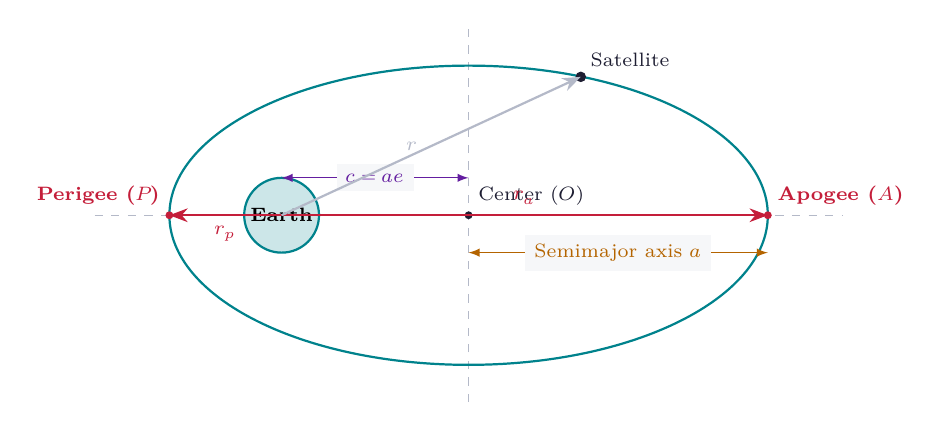
\begin{tikzpicture}[scale=0.95, every node/.style={font=\scriptsize}]
  % Draw axes
  \draw[dashed, color=mgframe] (-5.0,0) -- (5.0,0);
  \draw[dashed, color=mgframe] (0,-2.5) -- (0,2.5);
  
  % Draw Ellipse
  \draw[thick, color=myteal] (0,0) ellipse (4.0cm and 2.0cm);
  
  % Foci points
  \coordinate (F1) at (-2.5, 0); % Earth focus
  \coordinate (F2) at (2.5, 0);
  
  % Draw Earth at F1
  \fill[color=myteal!20, draw=myteal, line width=0.8pt] (F1) circle (0.5cm);
  \node at (F1) {\textbf{Earth}};
  
  % Center marker
  \fill[color=mydark] (0,0) circle (1.5pt) node[above right] {Center ($O$)};
  
  % Perigee and Apogee points
  \fill[color=myred] (-4.0,0) circle (1.5pt) node[above left, color=myred] {\textbf{Perigee ($P$)}};
  \fill[color=myred] (4.0,0) circle (1.5pt) node[above right, color=myred] {\textbf{Apogee ($A$)}};
  
  % Dimension lines
  % Semimajor axis 'a'
  \draw[latex-latex, color=myamber] (0,-0.5) -- node[midway, fill=mygray] {Semimajor axis $a$} (4.0,-0.5);
  % Focus distance 'ae'
  \draw[latex-latex, color=mypurple] (-2.5,0.5) -- node[midway, fill=mygray] {$c = ae$} (0,0.5);
  
  % Radius vectors
  \draw[arrow, color=myred] (F1) -- node[midway, below] {$r_p$} (-4.0,0);
  \draw[arrow, color=myred] (F1) -- node[midway, above] {$r_a$} (4.0,0);
  
  % Satellite on orbit
  \coordinate (Sat) at (1.5, 1.85);
  \fill[color=mydark] (Sat) circle (2pt) node[above right] {Satellite};
  \draw[arrow, color=mgframe] (F1) -- node[midway, left=0.05cm] {$r$} (Sat);
\end{tikzpicture}
\end{tcolorbox}

\subsection{Key Parameters and Formulas}
From the geometry of the ellipse:
\begin{enumerate}[label=\textbf{\arabic*.}, leftmargin=*, itemsep=3pt]
  \item \textbf{Perigee Distance ($r_p$):} The point of closest approach to the center of Earth.
    \begin{equation}
      r_p = a(1 - e)
    \end{equation}
  \item \textbf{Apogee Distance ($r_a$):} The point of farthest distance from the center of Earth.
    \begin{equation}
      r_a = a(1 + e)
    \end{equation}
  \item \textbf{Relationship to Altitudes:}
    \begin{equation}
      a = \frac{r_a + r_p}{2}
    \end{equation}
    \begin{equation}
      e = \frac{r_a - r_p}{r_a + r_p}
    \end{equation}
    Where $r_a = R_E + h_a$ and $r_p = R_E + h_p$ ($R_E \approx 6378 \text{ km}$ is Earth's mean radius, $h_a, h_p$ are apogee/perigee altitudes above Earth's surface).
\end{enumerate}

% ===============================================================================
\section{Orbital Equations and Parameters}
% ===============================================================================

The dynamics of a satellite are dictated by the balancing of gravitational and centripetal forces.

\subsection{Orbital Velocity}
The instantaneous velocity ($v$) of a satellite orbiting in an elliptical path at a distance $r$ from the center of Earth is given by the \textbf{Vis-Viva Equation}:
\begin{equation}
  v = \sqrt{\mu \left( \frac{2}{r} - \frac{1}{a} \right)}
\end{equation}

\begin{itemize}[leftmargin=*, itemsep=6pt]
  \item \textbf{For Circular Orbits ($r = a$):} The velocity remains constant at:
    \begin{equation}
      v_{c} = \sqrt{\frac{\mu}{r}}
    \end{equation}
  \item \textbf{At Perigee ($r = r_p = a(1-e)$):} The velocity is at its maximum:
    \begin{equation}
      v_{max} = \sqrt{\frac{\mu}{a}\left(\frac{1+e}{1-e}\right)}
    \end{equation}
  \item \textbf{At Apogee ($r = r_a = a(1+e)$):} The velocity is at its minimum:
    \begin{equation}
      v_{min} = \sqrt{\frac{\mu}{a}\left(\frac{1-e}{1+e}\right)}
    \end{equation}
\end{itemize}

\subsection{Angular Velocity}
The mean angular velocity ($\omega$) of a satellite in circular orbit (or the average mean motion $n$) is:
\begin{equation}
  \omega = \frac{2\pi}{T} = \sqrt{\frac{\mu}{a^3}}
\end{equation}
The instantaneous angular velocity at any distance $r$ is derived from conservation of angular momentum:
\begin{equation}
  \omega_{inst} = \frac{h}{r^2}
\end{equation}
Where $h = \sqrt{\mu a(1 - e^2)}$ is the specific angular momentum of the orbit.

% ===============================================================================
\section{Solar Day vs. Sidereal Day}
% ===============================================================================

To design satellite orbits that synchronize with Earth's rotation (like geostationary orbits), we must distinguish between two methods of measuring a day.

\begin{tcolorbox}[defbox]
\textbf{Solar Day:} The time taken for the Earth to rotate once about its axis relative to the Sun. It is exactly \textbf{24 hours} (86,400 seconds).

\textbf{Sidereal Day:} The time taken for the Earth to rotate once about its axis relative to the distant stars (inertial space). It is exactly \textbf{23 hours, 56 minutes, and 4.09 seconds} (86,164.09 seconds).
\end{tcolorbox}

\subsection{The Astronomical Difference}
Because the Earth orbits the Sun while rotating on its axis, it travels approximately $1^\circ$ along its orbital path each day. Consequently, the Earth must rotate slightly more than $360^\circ$ (about $360.986^\circ$) to bring the Sun back to the same meridian. A sidereal day is a true $360^\circ$ rotation.

\begin{tcolorbox}[tikzbox, title={Earth Rotation: Solar Day vs. Sidereal Day}]
\centering
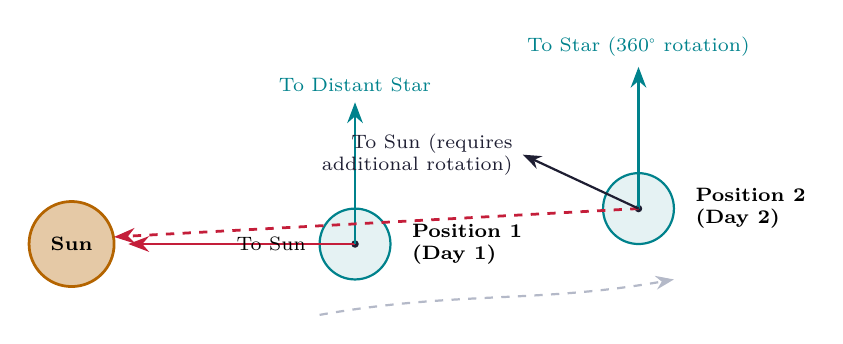
\begin{tikzpicture}[scale=0.9, every node/.style={font=\scriptsize}]
  % Sun (Left side)
  \fill[color=myamber!35, draw=myamber, line width=1.0pt] (-4,0) circle (0.6cm);
  \node at (-4,0) {\textbf{Sun}};
  
  % Earth Position 1 (Day 1)
  \coordinate (E1) at (0,0);
  \draw[thick, fill=myteal!10, draw=myteal] (E1) circle (0.5cm);
  \fill[color=mydark] (E1) circle (1.5pt);
  \node[right=0.6cm of E1, align=left] {\textbf{Position 1}\\\textbf{(Day 1)}};
  
  % Pointing vector to Sun and Star
  \draw[arrow, color=myred, line width=1pt] (E1) -- (-3.2,0);
  \draw[arrow, color=myteal, line width=1pt] (E1) -- (0,2) node[above] {To Distant Star};
  \node[left=0.5cm of E1] {To Sun};
  
  % Earth Position 2 (Day 2) after 360 rotation (Sidereal Day complete)
  \coordinate (E2) at (4,0.5);
  \draw[thick, fill=myteal!10, draw=myteal] (E2) circle (0.5cm);
  \fill[color=mydark] (E2) circle (1.5pt);
  \node[right=0.6cm of E2, align=left] {\textbf{Position 2}\\\textbf{(Day 2)}};
  
  % Pointing vectors at Position 2
  \draw[arrow, color=myteal, line width=1pt] (E2) -- (4,2.5) node[above] {To Star ($360^\circ$ rotation)};
  \draw[arrow, color=myred, line width=1pt, dashed] (E2) -- (-3.4,0.1); % Pointing to Sun
  \draw[arrow, color=mydark, line width=0.8pt] (E2) -- ($(E2)+(155:1.8)$) node[left, align=right] {To Sun (requires\\additional rotation)};
  
  % Orbit path
  \draw[arrow, dashed, color=mgframe] (-0.5,-1) to[out=10, in=190] (4.5,-0.5);
\end{tikzpicture}
\end{tcolorbox}

\subsection{Impact on Geostationary Orbit (GEO) Design}
A geostationary satellite must remain fixed relative to a point on the Earth. Therefore, its orbital period must match the Earth's inertial rotation rate, which is the \textbf{sidereal day} ($T = 86,164.09$ seconds), rather than the solar day.

Substituting $T = 86,164.09$ s into Kepler's Third Law:
\begin{equation}
  a^3 = \frac{T^2 \mu}{4\pi^2} = \frac{(86,164.09)^2 \times 3.986 \times 10^{14}}{4\pi^2} \approx 7.496 \times 10^{22} \text{ m}^3
\end{equation}
\begin{equation}
  a \approx 42,164 \text{ km}
\end{equation}
Subtracting Earth's equatorial radius ($R_E \approx 6,378$ km):
\begin{equation}
  h_{GEO} = a - R_E \approx 35,786 \text{ km}
\end{equation}
This derivation establishes the standard altitude of geostationary satellites.

% ===============================================================================
% MANDATORY QUICK REVISION PAGE
% ===============================================================================
\newpage
\begin{center}
  {\large\bfseries\color{myred} Quick Revision --- Module II}\\[3pt]
  {\small\color{mydark} Orbital Mechanics $|$ PE-EC701B}
\end{center}
\noindent{\color{myred}\rule{\linewidth}{1.2pt}}
\vspace{4pt}

\begin{tcolorbox}[formulabox, title={\textbf{Key Formulas at a Glance}}]
\renewcommand{\arraystretch}{1.9}
\begin{tabularx}{\linewidth}{B{5.0cm} X}
Kepler's Third Law & $\displaystyle T^2 = \frac{4\pi^2 a^3}{\mu}$ \quad ($\mu \approx 3.986 \times 10^{14} \text{ m}^3/\text{s}^2$) \\[4pt]
Vis-Viva (Velocity) Equation & $\displaystyle v = \sqrt{\mu\left(\frac{2}{r} - \frac{1}{a}\right)}$ \\[4pt]
Apogee \& Perigee Distance & $r_a = a(1 + e)$ \quad and \quad $r_p = a(1 - e)$ \\[4pt]
Eccentricity from Radii & $\displaystyle e = \frac{r_a - r_p}{r_a + r_p} = \frac{\sqrt{a^2 - b^2}}{a}$ \\[4pt]
Mean Motion / Angular Velocity & $\displaystyle \omega = \sqrt{\frac{\mu}{a^3}}$
\end{tabularx}
\end{tcolorbox}

\begin{tcolorbox}[defbox, title={\textbf{One-Line Definitions}}]
\begin{itemize}[leftmargin=*, itemsep=2.5pt, topsep=0pt]
  \item \textbf{Apogee:} The point in an orbit farthest from the center of the Earth.
  \item \textbf{Perigee:} The point in an orbit closest to the center of the Earth.
  \item \textbf{Eccentricity:} A parameter determining how much an orbit deviates from a perfect circle.
  \item \textbf{Vis-Viva Equation:} The direct mathematical relationship for velocity at any orbital radius.
  \item \textbf{Sidereal Day:} Time for Earth to rotate $360^\circ$ relative to distant stars (86,164.09 s).
  \item \textbf{Solar Day:} Time for Earth to align back with the Sun (86,400 s).
  \item \textbf{Geocentric Constant ($\mu$):} Product of Gravitational Constant $G$ and Mass of Earth $M_E$.
\end{itemize}
\end{tcolorbox}

\begin{tcolorbox}[exambox, title={\textbf{Frequently Asked / Viva Questions}}]
\begin{enumerate}[topsep=0pt, label=\textbf{Q\arabic*.}, itemsep=5pt]
  \item \Q{State Kepler's Second Law and explain its velocity implication.}
    A line joining a satellite and its primary sweeps out equal areas in equal times. Thus, velocity is not constant; the satellite accelerates as it approaches perigee and decelerates as it approaches apogee.
  \item \Q{Derive the orbital radius of a geostationary satellite.}
    Using Kepler's 3rd Law ($T^2 = 4\pi^2 a^3/\mu$) and substituting the sidereal day ($T = 86,164$ s) and $\mu = 3.986 \times 10^5 \text{ km}^3/\text{s}^2$, we get $a \approx 42,164$ km. Subtracting $R_E \approx 6,378$ km yields $h \approx 35,786$ km.
  \item \Q{What is the difference between a sidereal day and a solar day?}
    A sidereal day is measured relative to distant stars ($23\text{h }56\text{m }4\text{s}$), whereas a solar day is measured relative to the Sun ($24\text{h}$). The difference arises because the Earth moves along its orbit around the Sun.
  \item \Q{Define eccentricity ($e$) and state its values for circular, elliptical, parabolic, and hyperbolic trajectories.}
    Eccentricity defines orbital shape. Circle: $e = 0$; Ellipse: $0 < e < 1$; Parabola: $e = 1$ (escape trajectory); Hyperbola: $e > 1$.
  \item \Q{Where is the satellite velocity maximum and minimum, and what are the expressions?}
    Maximum at perigee: $v_{max} = \sqrt{\frac{\mu}{a}\left(\frac{1+e}{1-e}\right)}$. Minimum at apogee: $v_{min} = \sqrt{\frac{\mu}{a}\left(\frac{1-e}{1+e}\right)}$.
  \item \Q{What is the physical significance of the geocentric gravitational constant ($\mu$)?}
    It is the product $G \cdot M_E$ (approx $3.986 \times 10^{14} \text{ m}^3/\text{s}^2$). It simplifies orbital math by combining the mass of the primary body and the gravitational constant.
  \item \Q{Why does a satellite not fall to Earth if gravity is constantly pulling it?}
    The satellite's high tangential velocity creates a centrifugal effect that balances the Earth's gravitational pull. It is in a continuous state of free fall around Earth's curve.
  \item \Q{An elliptical orbit has $r_p = 7,000$ km and $r_a = 15,000$ km. Calculate the semimajor axis and eccentricity.}
    $a = (r_a + r_p)/2 = 11,000$ km. $e = (r_a - r_p)/(r_a + r_p) = (15000-7000)/(15000+7000) = 8/22 \approx 0.364$.
  \item \Q{How does the orbital period change if the altitude of a satellite is doubled?}
    Since $T \propto a^{1.5}$, if $a$ increases, the period $T$ increases by $2^{1.5} \approx 2.83$ times.
  \item \Q{What is specific angular momentum ($h$) of an orbit?}
    It is the angular momentum per unit mass, $h = r \times v$. It remains constant along the orbit, demonstrating Kepler's second law.
  \item \Q{What is the escape velocity from Earth's surface?}
    $v_{esc} = \sqrt{2gR_E} = \sqrt{2\mu/R_E} \approx 11.2 \text{ km/s}$.
  \item \Q{How does body eccentricity impact solar day length?}
    If Earth's orbit eccentricity were larger, the orbital speed around the Sun would vary more, causing the solar day duration to fluctuate significantly throughout the year.
\end{enumerate}
\tcbset{colbacktitle=myteal, coltitle=white}
\end{tcolorbox}

\begin{tcolorbox}[tikzbox, title={Comparison of Earth Orbit Altitudes}]
\renewcommand{\arraystretch}{1.4}
\par\noindent
\begin{tabularx}{\linewidth}{|B{3.2cm}|Y|Y|Y|}
\hline
\rowcolor{hdrgray}
\textbf{Orbit Class} & \textbf{Typical Altitude ($h$)} & \textbf{Orbital Period ($T$)} & \textbf{Primary Application} \\
\hline
\textbf{LEO (Low Earth)} & $160 - 2,000$ km & $90 - 120$ minutes & Earth imaging, ISS, Starlink satellite constellations. \\
\hline
\rowcolor{rowalt}
\textbf{MEO (Medium Earth)} & $2,000 - 35,000$ km & $2 - 24$ hours & GPS (~12 hours), Galileo navigation constellations. \\
\hline
\textbf{GEO (Geostationary)} & $35,786$ km & $23\text{h }56\text{m }4\text{s}$ (Sidereal) & Weather satellites, satellite TV broadcast, VSAT links. \\
\hline
\rowcolor{rowalt}
\textbf{HEO (Highly Elliptical)} & $1,000 - 40,000$ km (Molniya) & ~$12$ hours & Communication at high polar latitudes (Russian Molniya). \\
\hline
\end{tabularx}
\end{tcolorbox}

\end{document}
